%Version 3.1 December 2024
% See section 11 of the User Manual for version history
%
%%%%%%%%%%%%%%%%%%%%%%%%%%%%%%%%%%%%%%%%%%%%%%%%%%%%%%%%%%%%%%%%%%%%%%
%%                                                                 %%
%% Please do not use \input{...} to include other tex files.       %%
%% Submit your LaTeX manuscript as one .tex document.              %%
%%                                                                 %%
%% All additional figures and files should be attached             %%
%% separately and not embedded in the \TeX\ document itself.       %%
%%                                                                 %%
%%%%%%%%%%%%%%%%%%%%%%%%%%%%%%%%%%%%%%%%%%%%%%%%%%%%%%%%%%%%%%%%%%%%%

%%\documentclass[referee,sn-basic]{sn-jnl}% referee option is meant for double line spacing

%%=======================================================%%
%% to print line numbers in the margin use lineno option %%
%%=======================================================%%

%%\documentclass[lineno,pdflatex,sn-basic]{sn-jnl}% Basic Springer Nature Reference Style/Chemistry Reference Style

%%=========================================================================================%%
%% the documentclass is set to pdflatex as default. You can delete it if not appropriate.  %%
%%=========================================================================================%%

%%\documentclass[sn-basic]{sn-jnl}% Basic Springer Nature Reference Style/Chemistry Reference Style

%%Note: the following reference styles support Namedate and Numbered referencing. By default the style follows the most common style. To switch between the options you can add or remove “Numbered” in the optional parenthesis. 
%%The option is available for: sn-basic.bst, sn-chicago.bst%  
 
%%\documentclass[pdflatex,sn-nature]{sn-jnl}% Style for submissions to Nature Portfolio journals
%%\documentclass[pdflatex,sn-basic]{sn-jnl}% Basic Springer Nature Reference Style/Chemistry Reference Style
\documentclass[pdflatex,sn-mathphys-num]{sn-jnl}% Math and Physical Sciences Numbered Reference Style
%%\documentclass[pdflatex,sn-mathphys-ay]{sn-jnl}% Math and Physical Sciences Author Year Reference Style
%%\documentclass[pdflatex,sn-aps]{sn-jnl}% American Physical Society (APS) Reference Style
%%\documentclass[pdflatex,sn-vancouver-num]{sn-jnl}% Vancouver Numbered Reference Style
%%\documentclass[pdflatex,sn-vancouver-ay]{sn-jnl}% Vancouver Author Year Reference Style
%%\documentclass[pdflatex,sn-apa]{sn-jnl}% APA Reference Style
%%\documentclass[pdflatex,sn-chicago]{sn-jnl}% Chicago-based Humanities Reference Style

%%%% Standard Packages
%%<additional latex packages if required can be included here>

\usepackage{graphicx}%
\usepackage{multirow}%
\usepackage{amsmath,amssymb,amsfonts}%
\usepackage{amsthm}%
\usepackage{mathrsfs}%
\usepackage[title]{appendix}%
\usepackage{xcolor}%
\usepackage{textcomp}%
\usepackage{manyfoot}%
\usepackage{booktabs}%
\usepackage{algorithm}%
\usepackage{algorithmicx}%
\usepackage{algpseudocode}%
\usepackage{listings}
\usepackage{natbib}
\usepackage{cleveref}
\usepackage{dirtytalk}
\usepackage{subcaption}
\usepackage{wrapfig}
\usepackage{caption}
\captionsetup[figure]{font=footnotesize}
\usepackage{float}
%
%%%%

%%%%%=============================================================================%%%%
%%%%  Remarks: This template is provided to aid authors with the preparation
%%%%  of original research articles intended for submission to journals published 
%%%%  by Springer Nature. The guidance has been prepared in partnership with 
%%%%  production teams to conform to Springer Nature technical requirements. 
%%%%  Editorial and presentation requirements differ among journal portfolios and 
%%%%  research disciplines. You may find sections in this template are irrelevant 
%%%%  to your work and are empowered to omit any such section if allowed by the 
%%%%  journal you intend to submit to. The submission guidelines and policies 
%%%%  of the journal take precedence. A detailed User Manual is available in the 
%%%%  template package for technical guidance.
%%%%%=============================================================================%%%%

%% as per the requirement new theorem styles can be included as shown below
\theoremstyle{thmstyleone}%
\newtheorem{theorem}{Theorem}%  meant for continuous numbers
%%\newtheorem{theorem}{Theorem}[section]% meant for sectionwise numbers
%% optional argument [theorem] produces theorem numbering sequence instead of independent numbers for Proposition
\newtheorem{proposition}[theorem]{Proposition}% 
%%\newtheorem{proposition}{Proposition}% to get separate numbers for theorem and proposition etc.

\theoremstyle{thmstyletwo}%
\newtheorem{example}{Example}%
\newtheorem{remark}{Remark}%

\theoremstyle{thmstylethree}%
\newtheorem{definition}{Definition}%

\raggedbottom
%%\unnumbered% uncomment this for unnumbered level heads

\begin{document}

\title[Title]{Manifold Learning for Dyanmics Aware Reward Modeling in Reinforcement Learning}

\author*[1]{\fnm{Joshua} \sur{Groves}}\email{groves.152@osu.edu}

\author[1]{\fnm{Michael} \sur{Groeber}}\email{groeber.9@osu.edu}

\affil*[1]{\orgdiv{Integrated Systems Engineering}, \orgname{The Ohio State University}, \orgaddress{\street{210 Baker Systems Bldg., 1971 Neil Avenue}, \city{Columbus}, \postcode{43210}, \state{OH}, \country{USA}}}

\abstract{Applied reinforcement learning (RL) is a difficult task in-part due to the meticulous reward engineering required to steer agents toward optimal policies \cite{rewmodelsurvey}. Attempts have been made to utilize foundational models such as LLMs to iteratively design reward functions - while these are effective running such LLMs require expensive hardware, may be difficult to integrate tightly with the RL training loop,  may be untrustworthy and may not be grounded in physical priors of the environment. We propose a manifold learning approach which utilizes Uniform Manifold Approximate Project to  maps state transitions onto an \(n\)-dimensional manifold. Assuming such transitions are physically governed and preserve a Riemannian metric the resulting manifold preserves a notion of distance which we leverage as our reward model. This approach can be utilized for solving Markov Decision Processes which have easily identifiable (but difficult to specify) reward states. Empirically, we show that over three toy gymnasium environments, the learned reward model improves sample efficiency of the agent when the learned manifold is maps state transitions which coorelate to optimal policy behaviour. Additionally, we show that with little impact to the sample effiency we learn the reward model online jointly with policy learning.}


\keywords{reinforcement learning, manifold, umap}

%%\pacs[JEL Classification]{D8, H51}

%%\pacs[MSC Classification]{35A01, 65L10, 65L12, 65L20, 65L70}

\maketitle

\section{Introduction}\label{sec1}



\subsection{Related Work}



\section{Methodology}



\section{Results and Discussion}\label{sec12}

\section{Conclusion}\label{sec13}

\bmhead{Acknowledgements}


\section*{Declarations}

\bmhead{Conflicts of Interest} The authors declare no conflict of interest.

\bmhead{Data Availability} Data can be provided upon request. Code is available at \url{https://github.com/OSU-SIMCenter/forge-net}


%%===================================================%%
%% For presentation purpose, we have included        %%
%% \bigskip command. Please ignore this.             %%
%%===================================================%%
\bigskip
\begin{flushleft}%
Editorial Policies for:

\bigskip\noindent
Springer journals and proceedings: \url{https://www.springer.com/gp/editorial-policies}

\bigskip\noindent
Nature Portfolio journals: \url{https://www.nature.com/nature-research/editorial-policies}

\bigskip\noindent
\textit{Scientific Reports}: \url{https://www.nature.com/srep/journal-policies/editorial-policies}

\bigskip\noindent
BMC journals: \url{https://www.biomedcentral.com/getpublished/editorial-policies}
\end{flushleft}

\newpage
\begin{appendices}

\section{Rollout Predictions Standard Deviations}\label{sec:std_deviation}

\cref{fig:rollout_compare_appendix} demonstrates further that the chamfer trained model achieves accurate one-step predictions with low variance in the predictions for a variety of hits but quickly accumulates error, surpassing the worst case error of the MSE model on the recursive rollout test after only 15 steps. Comparatively, the MSE models' worst \(5\%\) of points are only 0.2 units off even after 50 recursive predictions.

\begin{figure}[htbp]
\centering
  \begin{subfigure}[b]{1.0\textwidth} % Increased width for better visibility
    \centering
    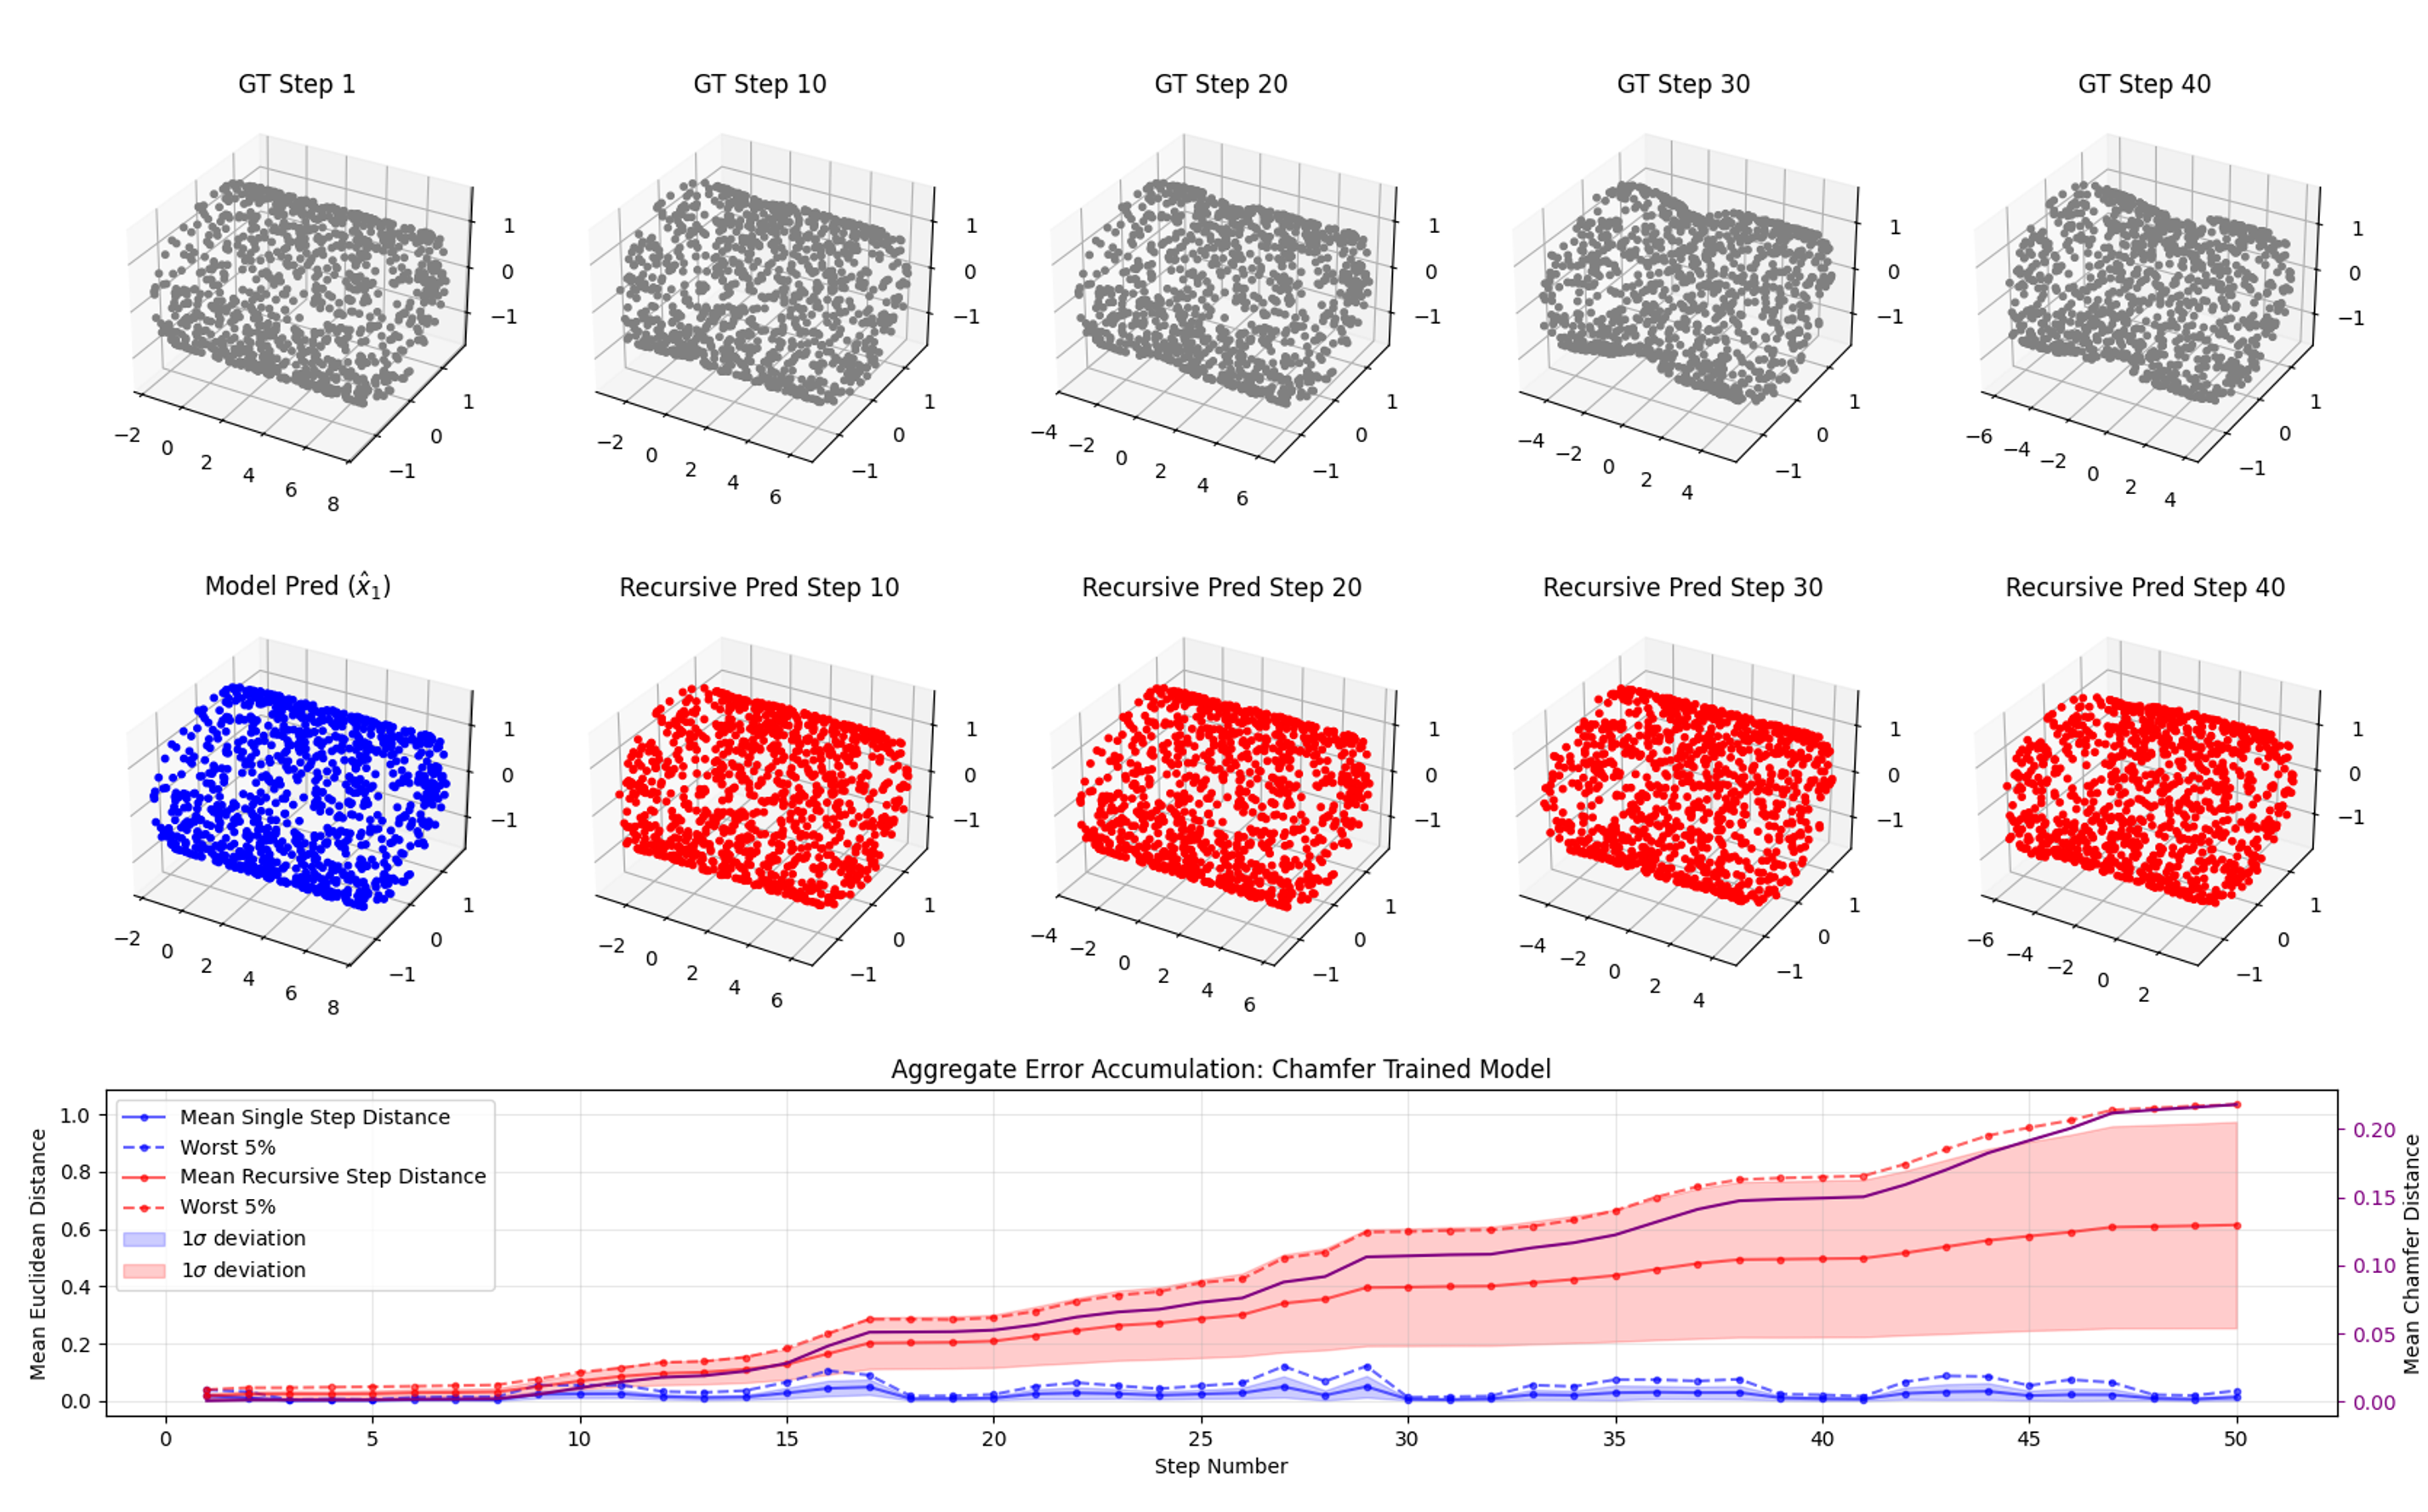
\includegraphics[width=\textwidth]{figures/eval_series_chamfer.png}
  \end{subfigure}
  \\ % This forces the vertical stack
  \begin{subfigure}[b]{1.0\textwidth}
    \centering
    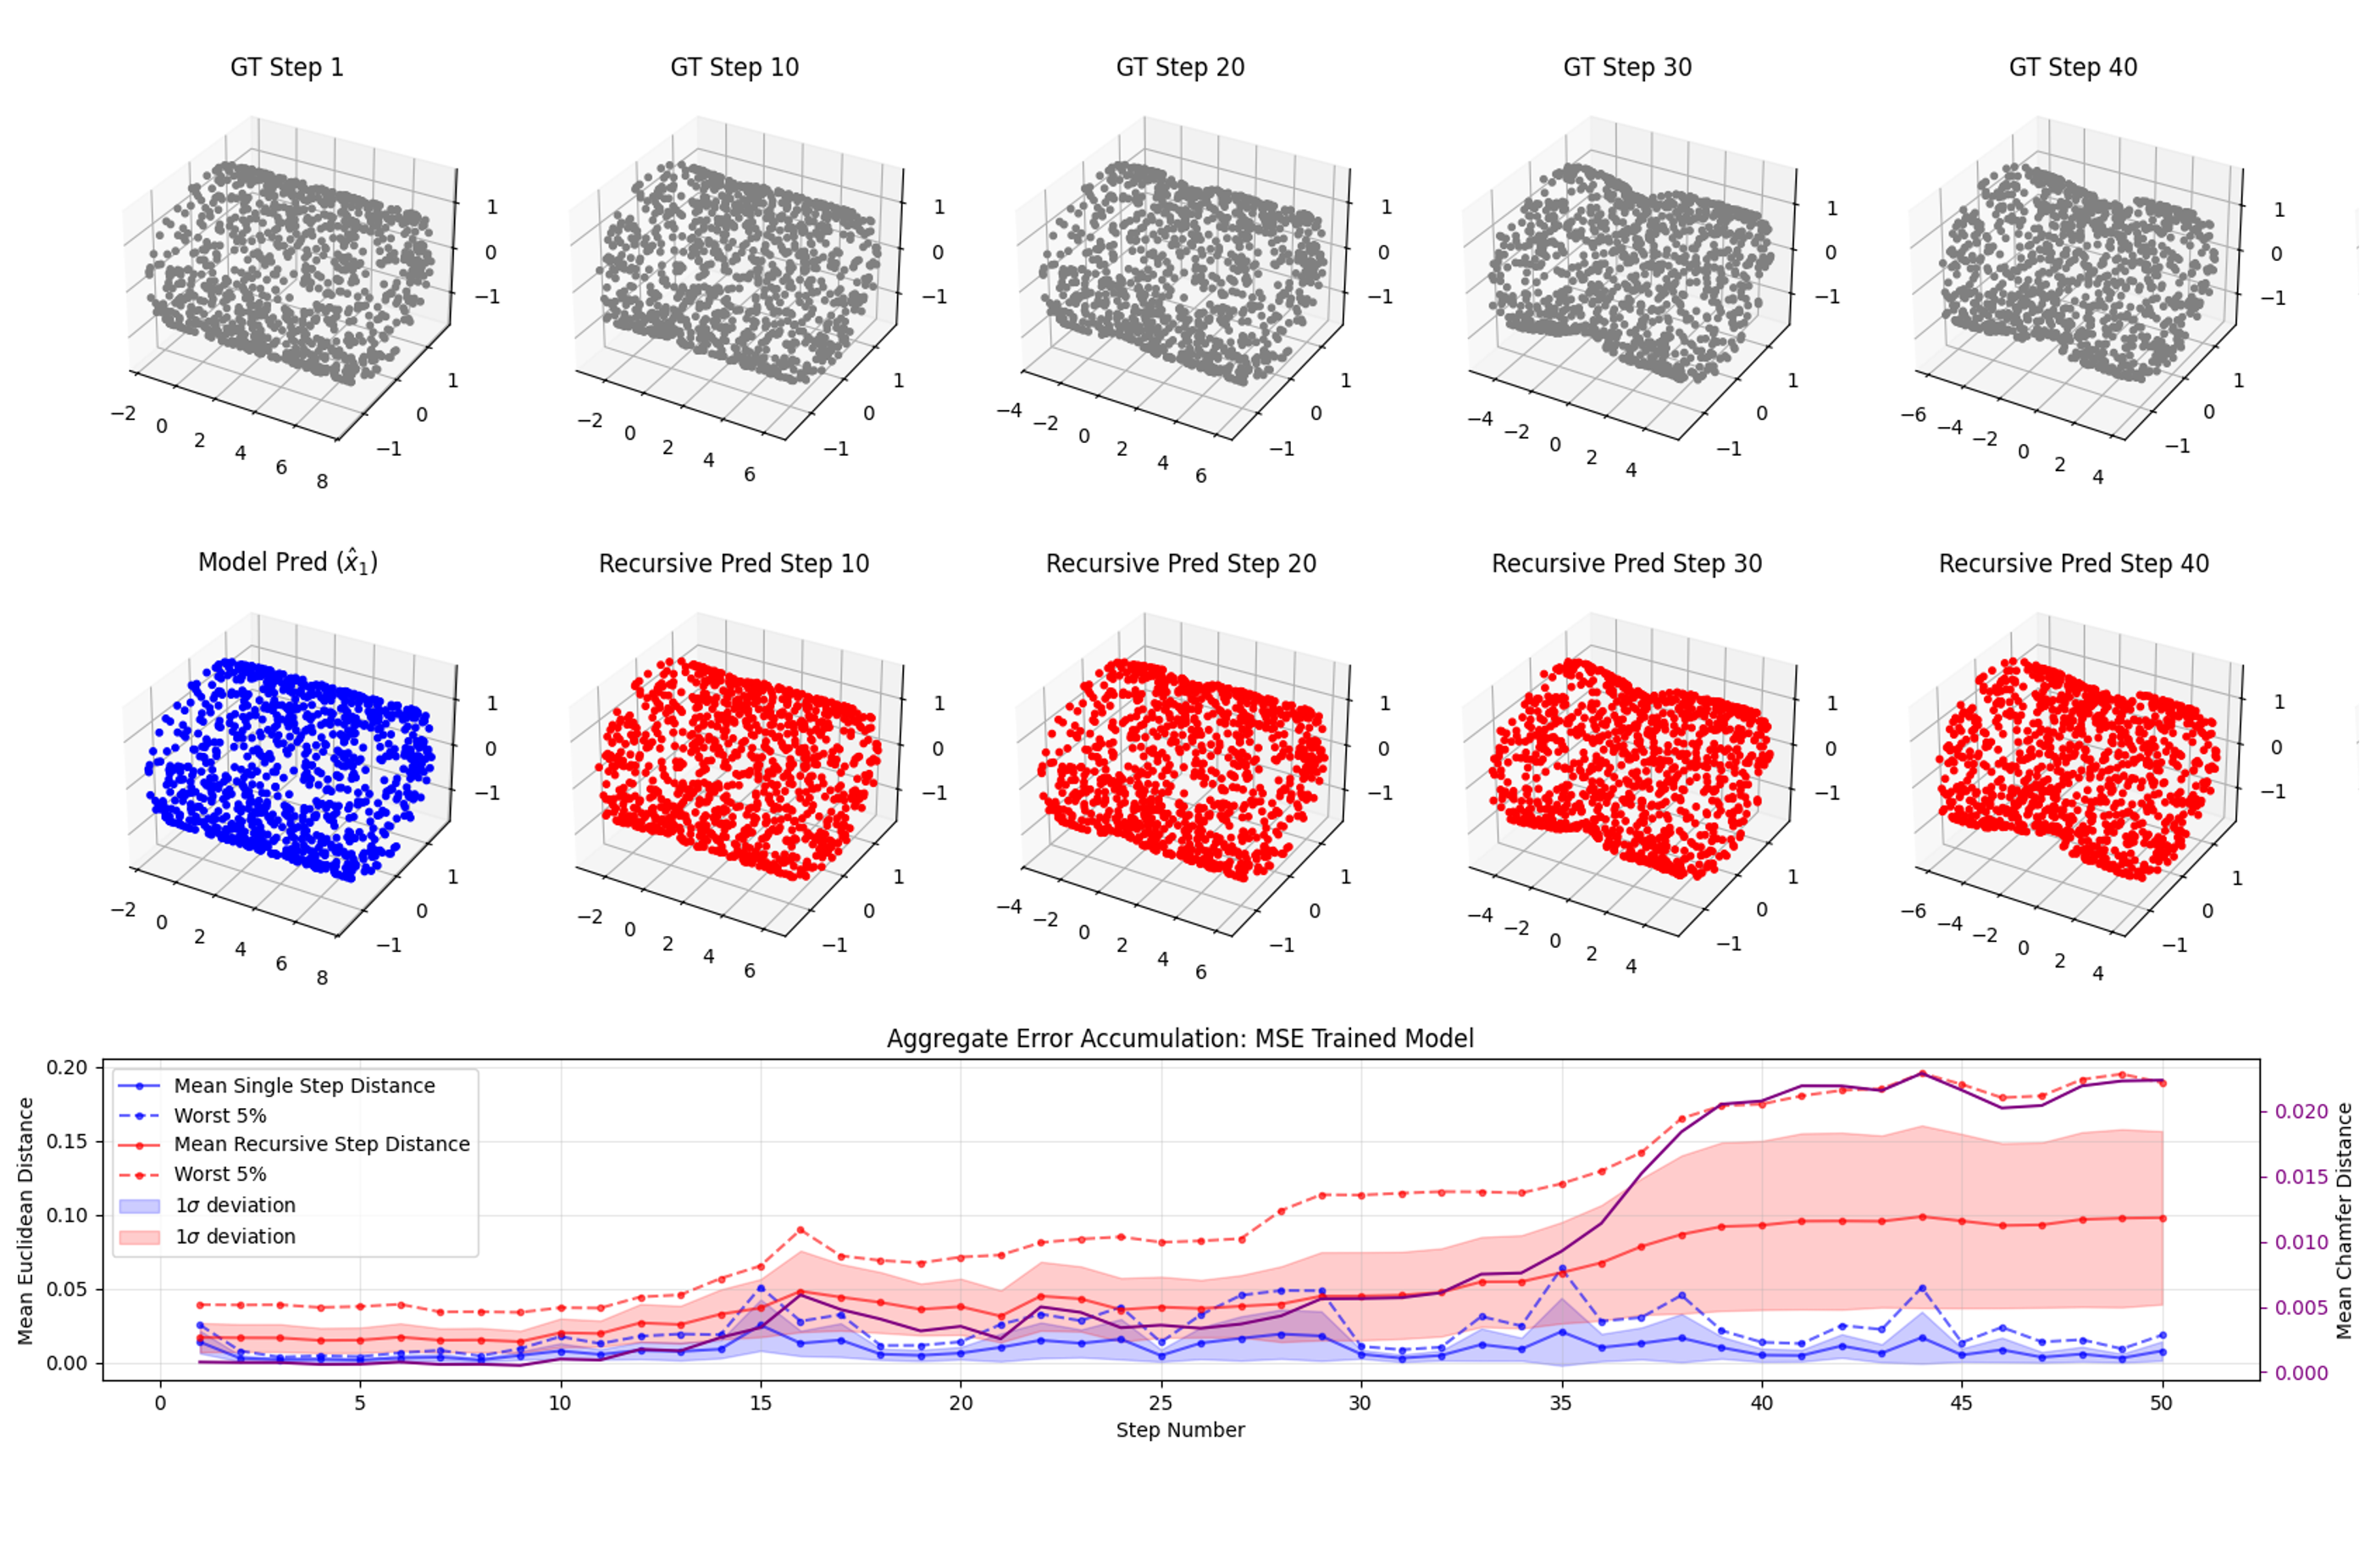
\includegraphics[width=\textwidth]{figures/eval_series_mse.png}
  \end{subfigure}
\caption{Point cloud predictions and reconstruction performance plots for chamfer trained model (top) and MSE trained model (bottom). MED scores are shwon for one-step (blue) and recursive rollout (red) performance. Chamfer discrepancy is shown in purple.}
\label{fig:rollout_compare_appendix}
\end{figure}

\newpage
\section{Barycentric Mesh Sampling for Dataset Generation}\label{sec:barycentric_sampling}

\begin{algorithm}
\caption{Area-Weighted Barycentric Mesh Sampling}
\label{alg:barycentric_sampling}
\begin{algorithmic}[1]
\Statex \textbf{Input:} Mesh $\mathcal{M}$, sample count $N$, seed $\zeta$
\Statex \textbf{Output:} Sampled points $\mathcal{P}$, original triangle indices $\mathcal{I}_{orig}$, barycentric coordinates $\mathcal{B}$
\State Initialize RNG with $\zeta$
\State $\mathcal{T} \gets \text{Faces}(\mathcal{M})$
\State $\mathcal{A} \gets \text{CellAreas}(\mathcal{M})$
\State $\mathcal{I} \gets \{0, 1, \dots, |\mathcal{T}|-1\}$ \Comment{Original global indices}
\State $A_{total} \gets \sum \mathcal{A}$
\State $\mathcal{P}, \mathcal{I}_{orig}, \mathcal{B} \leftarrow \emptyset$
\State
\For{$i = 1$ \textbf{to} $N$}
    \State $j \gets \text{Sample index from } \mathcal{I} \text{ with probability } \mathcal{A}/A_{total}$
    \State $(v_0, v_1, v_2) \gets \text{Vertices of } \mathcal{T}[j]$
    \State $r_0, r_1 \sim \mathcal{U}(0, 1)$ \Comment{Uniform random variables}
    \State
    \State $b_0 \leftarrow 1 - \sqrt{r_0}$ \Comment{Square root for uniform distribution}
    \State $b_1 \leftarrow \sqrt{r_0}(1 - r_1)$
    \State $b_2 \leftarrow r_1\sqrt{r_0}$
    \State
    \State $\mathbf{p} \leftarrow b_0 v_0 + b_1 v_1 + b_2 v_2$
    \State
    \State $\mathcal{P} \leftarrow \mathcal{P} \cup \{\mathbf{p}\}$
    \State $\mathcal{I}_{orig} \leftarrow \mathcal{I}_{orig} \cup \{\mathcal{I}[j]\}$
    \State $\mathcal{B} \leftarrow \mathcal{B} \cup \{(b_0, b_1, b_2)\}$
\EndFor
\State \Return $\mathcal{P}, \mathcal{I}_{orig}, \mathcal{B}$
\end{algorithmic}
\end{algorithm}

\section{ForgeNet: Full architecture details}\label{sec:architecture}

The ForgeNet model is implemented as a conditional autoencoder designed to predict point-wise displacement fields \(\Delta \in \mathbb{R}^{N \times 3}\) for a fixed cardinality of N=2048 vertices. The architecture comprises two encoding heads—a state encoder and an action encoder—that map inputs into a shared latent space. The state encoder processes the input point cloud of shape \(3 \times N\) through a series of five 1D convolutional layers with unit kernel sizes and channel widths of 64, 64, 128, 256, and 256, respectively. Each layer is followed by batch normalization and ReLU activation. A global max-pooling operation is applied across the point dimension to extract a 256-dimensional permutation-invariant feature vector. Simultaneously, the action encoder processes a 1-dimensional action feature (simulation steps) through a five-layer MLP with widths of 64, 64, 128, 256, and 256.

The resulting latent vectors are concatenated into a 512-dimensional global context vector, which is subsequently tiled and augmented with the original XYZ coordinates to form a $(512+3) \times N$ feature map. 
The decoder employs four 1D convolutional layers with widths of 512, 256, 128, and 3 to map these features back to the spatial domain. For this configuration, residual connections were disabled as we did not see any accuracy improvements with them enabled. We leave them in our implementation however for later iterations where they may be beneficial. To ensure reproducibility, weights were initialized via the Kaiming normal method and trained using the Adam optimizer with a base learning rate of \(1.0 \times 10^{-4} \), a weight decay of \(1.0 \times 10^{-2} \), and a dropout probability of 0.1. The network was optimized to minimize the Mean Squared Error (MSE) between the predicted and ground-truth vertex displacements.

\section{Mesh Reconstruction}\label{sec:mesh_recon}

To provide visual intuition for ForgeNet's ability to accurately predict forging deformations we setup a LSQR problem (using Scipy's provded LSQR package) to reconstruct the mesh with new vertex positions given predicted barycentric coordinate locations. \cref{fig:mesh_recon} show the original deformed mesh from JAX-Forge and the resulting reconstructed mesh given the predicted barycentric coordinate deltas from ForgeNet.


\begin{figure}[H]
 \begin{center}
 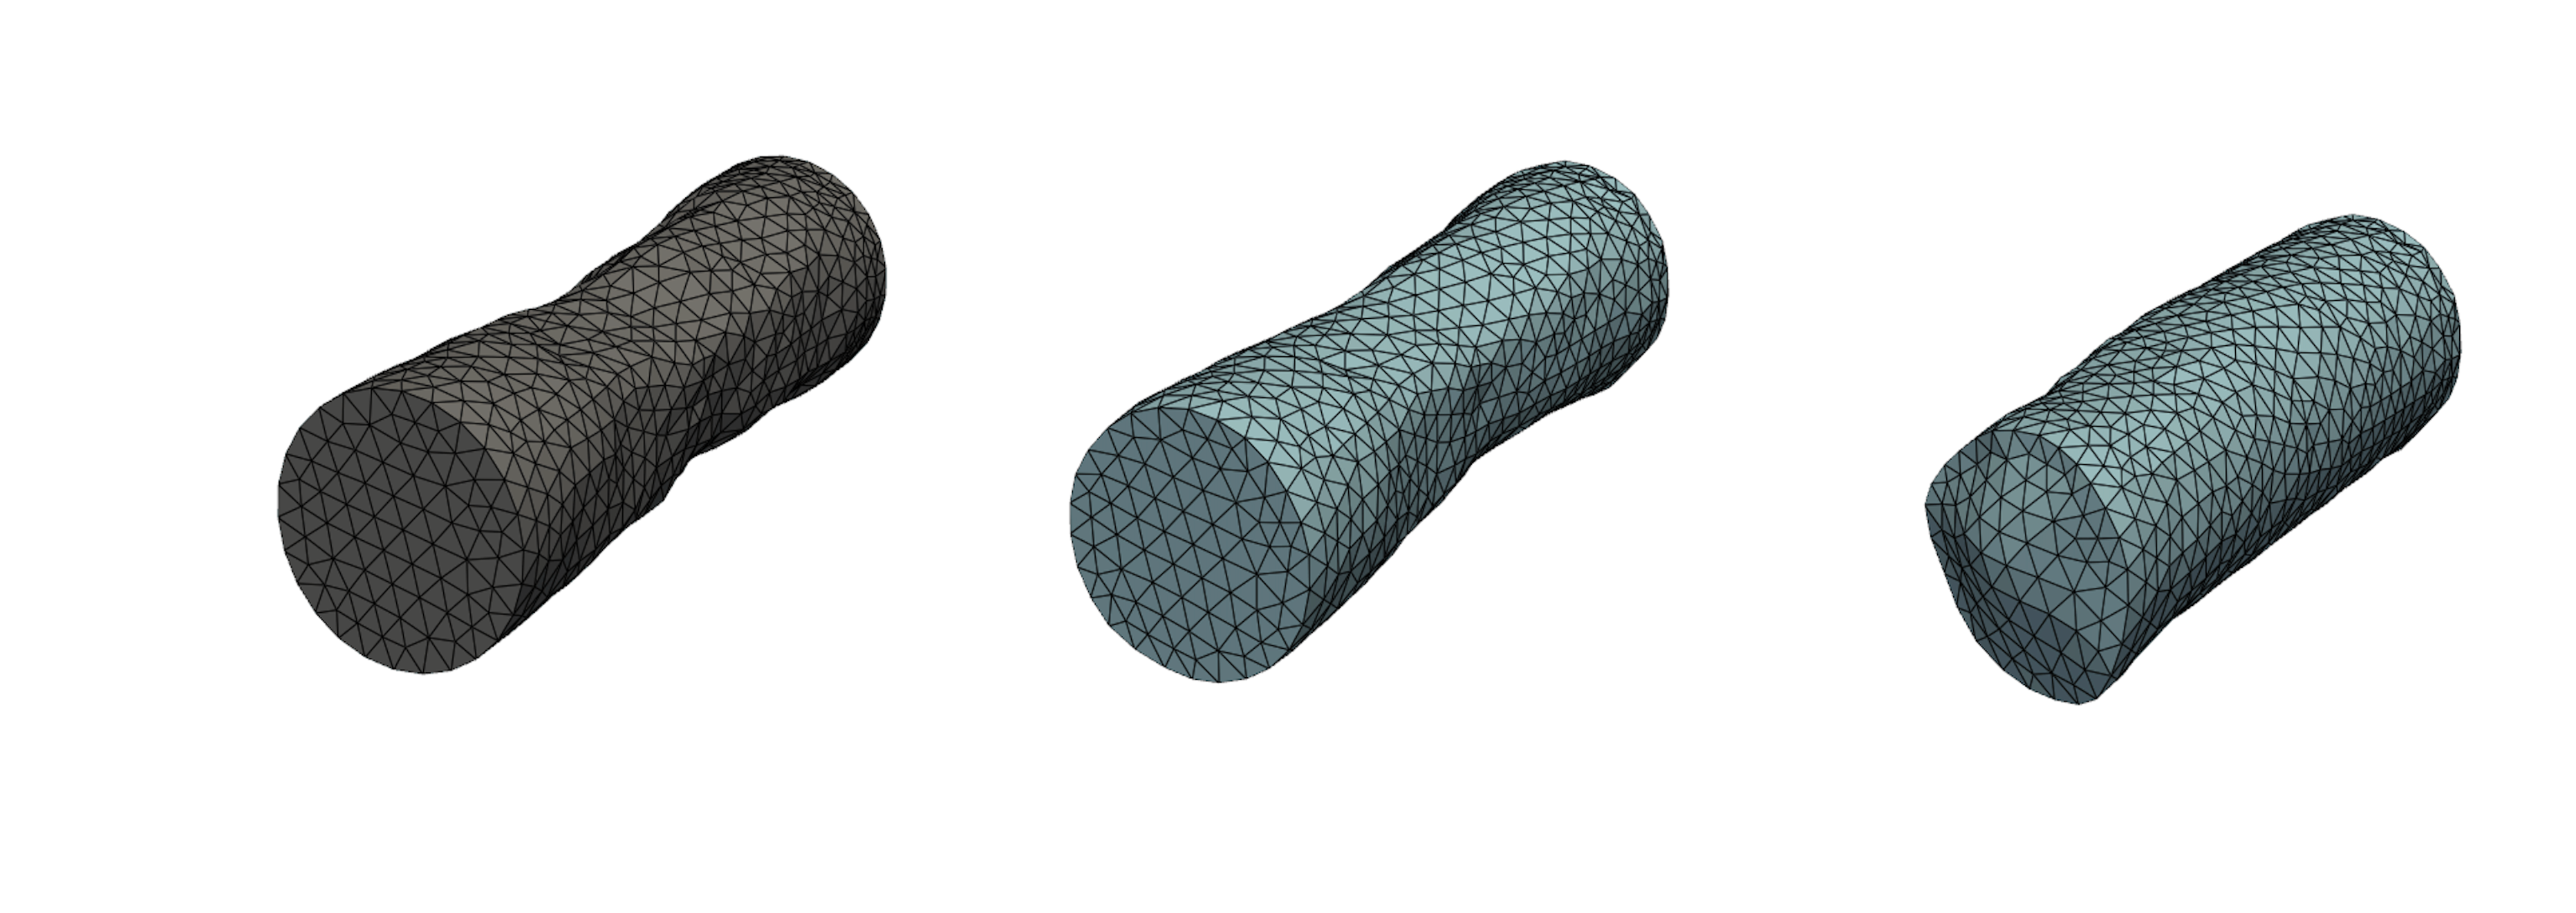
\includegraphics[width=1.0\textwidth]{figures/mesh_recon.png}
  \caption{Ground truth surface mesh (left). Reconstructed surface mesh from MSE traiend network network prediction (middle) Reconstruction from chamfer trained network prediction (right).}
  \label{fig:mesh_recon}
 \end{center}
\end{figure}


\end{appendices}

%%===========================================================================================%%
%% If you are submitting to one of the Nature Portfolio journals, using the eJP submission   %%
%% system, please include the references within the manuscript file itself. You may do this  %%
%% by copying the reference list from your .bbl file, paste it into the main manuscript .tex %%
%% file, and delete the associated \verb+\bibliography+ commands.                            %%
%%===========================================================================================%%
\newpage
\bibliography{sn-bibliography.bib}% common bib file
%% if required, the content of .bbl file can be included here once bbl is generated
%%\input sn-article.bbl

\end{document}
